\section{QUADCÓPTERO: SNAP ROLL}

% ============================================================
\begin{frame}{P2: Modelo Dinámico del Quadcoptero}
\begin{columns}[T]
\begin{column}{0.50\textwidth}
\begin{tbox}{Estados y Actuación}
\footnotesize
\textbf{Estado} $\bx \in \RR^{12}$ y \textbf{Control} $\bu \in \RR^4$:
\begin{align*}
\bx &= \begin{bmatrix}\bp\tr & \bm{\eta}\tr & \bv\tr & \bomega\tr\end{bmatrix}\tr\\
\bu &= \begin{bmatrix}F & \tau_x & \tau_y & \tau_z\end{bmatrix}\tr
\end{align*}
\begin{itemize}
\item $F$: empuje total a lo largo del eje $z$ del cuerpo.
\item $\btau = (\tau_x,\tau_y,\tau_z)$: momentos de control.
\item Parámetros: $m=1$\,kg, $I=\mathrm{diag}(0.02, 0.02, 0.04)\,\text{kg}\cdot\text{m}^2$.
\end{itemize}
\end{tbox}
\end{column}

\begin{column}{0.46\textwidth}
\begin{tbox}{Dinámica SE(3)}
\footnotesize
\begin{align*}
\dot{\bp} &= \bv \\
m\dot{\bv} &= F\,\bR(\bm{\eta})\mathbf{e}_3 - mg\,\mathbf{e}_3 \\
\dot{\bm{\eta}} &= E(\phi,\theta)\,\bomega \\
I\dot{\bomega} &= \btau - \bomega \times (I\bomega)
\end{align*}
\begin{itemize}
\item Orientación por ángulos Euler ZYX.
\item Se acota $|\theta| \le \theta_{\max} = 0.55$\,rad ($\approx 31.5^\circ$) para evitar la singularidad del gimbal lock.
\end{itemize}
\end{tbox}
\end{column}
\end{columns}
\src{Condiciones: $\bp_0=(0,0,1)$\,m a $\bp_f=(4,2,1.3)$\,m en $T=6$\,s con $\psi_f=90^\circ$}
\end{frame}

% ============================================================
\begin{frame}{P2: Geometría de la Pared y Maniobra Invertida}
\begin{columns}[T]
\begin{column}{0.50\textwidth}
\begin{tbox}{Geometría de la Ventana}
\small
Pared en $x_w=2$\,m (espesor $e=0.06$\,m) con orificio centrado en $\bm{c}_h = (2, 1, 1)$\,m:
\begin{equation*}
|y - y_h| \le a,\quad |z - z_h| \le b
\end{equation*}
con semiancho $a=0.32$\,m y semialtura $b=0.25$\,m.
\vskip4pt
Brazos del quad: $\ell=0.17$\,m, radio rotores $r_r=0.03$\,m.
\end{tbox}
\end{column}

\begin{column}{0.46\textwidth}
\begin{tbox}{Ventaja del Snap Roll}
\small
\begin{itemize}
\item Al cruzar boca abajo ($\phi = 180^\circ = \pi$):
\begin{equation*}
\bm{b}_2 \cdot \mathbf{e}_3 \approx 0
\end{equation*}
\item El brazo transversal se alinea horizontalmente con la apertura ancha ($a=0.32$\,m).
\item Permite atravesar un hueco de $0.50$\,m de altura sin colisión.
\end{itemize}
\end{tbox}
\end{column}
\end{columns}
\end{frame}

% ============================================================
\begin{frame}{P2: Problema de control óptimo}
\begin{columns}[T]
\begin{column}{0.46\textwidth}
\begin{tbox}{Restricciones en el problema}
\footnotesize
\begin{align*}
\min_{\bx(\cdot),\bu(\cdot)}\quad & J=\int_0^T \ell_c(\bx,\bu)\,dt\\
\text{s.a.}\quad & \dot\bx=\bm f(\bx,\bu),\\
& \bx(0)=\bx_0,\\
& \bx(T)=\bx_f=[\bp_f,\,(2\pi,0,\tfrac{\pi}{2}),\,\mathbf 0],\\
& \\
& 0\le F\le 2mg,\\
& \tau_{\min}\le \tau\le \tau_{\max},\\
& z_{\min}\le z\le z_{\max},\\
& \phi_{\min}\le\phi\le\phi_{\max},\\
& \phi(t_c)=\pi,\\
\end{align*}
\vspace{-8mm}
\end{tbox}
\end{column}

\begin{column}{0.48\textwidth}
\begin{tbox}
\footnotesize
\vspace{-3mm}
\footnotesize
\begin{align*}
& \text{si }|x-x_w|\le e/2:\\
& \quad \big|(y-y_h)\pm\ell\,\bm b_i\!\cdot\!\mathbf e_2\big|\le a-r_r,\\
& \quad \big|(z-z_h)\pm\ell\,\bm b_i\!\cdot\!\mathbf e_3\big|\le b-r_r,\ \ i=1,2.
\end{align*}
\end{tbox}
\end{column}
\end{columns}
\end{frame}


\begin{frame}{P2: Formulación del NLP (Multiple Shooting)}
    \begin{tbox}{Función de costo discreta}
    \small
    \begin{multline*}
    J=\sum_{k=0}^{N-1}h\Big[2\|\bp_k-\bp_{\mathrm{ref},k}\|^2+0.02\|\bv_k\|^2+0.5\,\theta_k^2\\
    +0.05(\phi_k-\phi_{\mathrm{ref},k})^2+0.12(\psi_k-\psi_{\mathrm{ref},k})^2+0.035\|\bomega_k\|^2\\
    +0.025(F_k-mg)^2+0.25\|\btau_k\|^2\Big]+0.02\sum_{k=1}^{N-1}\|\bu_k-\bu_{k-1}\|^2 .
    \end{multline*}
    \end{tbox}
    \begin{pbox}
    \footnotesize
    \textbf{Función de Costo:} Penaliza desviaciones de trayectoria de referencia (curvas quinticas / Hermite), minimiza esfuerzo de empuje $(F-mg)^2$, momento $\|\btau\|^2$ y variaciones suaves de control $\|\Delta \bu\|^2$.
    \end{pbox}
\end{frame}


% ============================================================
\begin{frame}{P2: Resultados -- Trayectoria y Maniobra 3D}
\begin{columns}[c]
\begin{column}{0.54\textwidth}
\centering
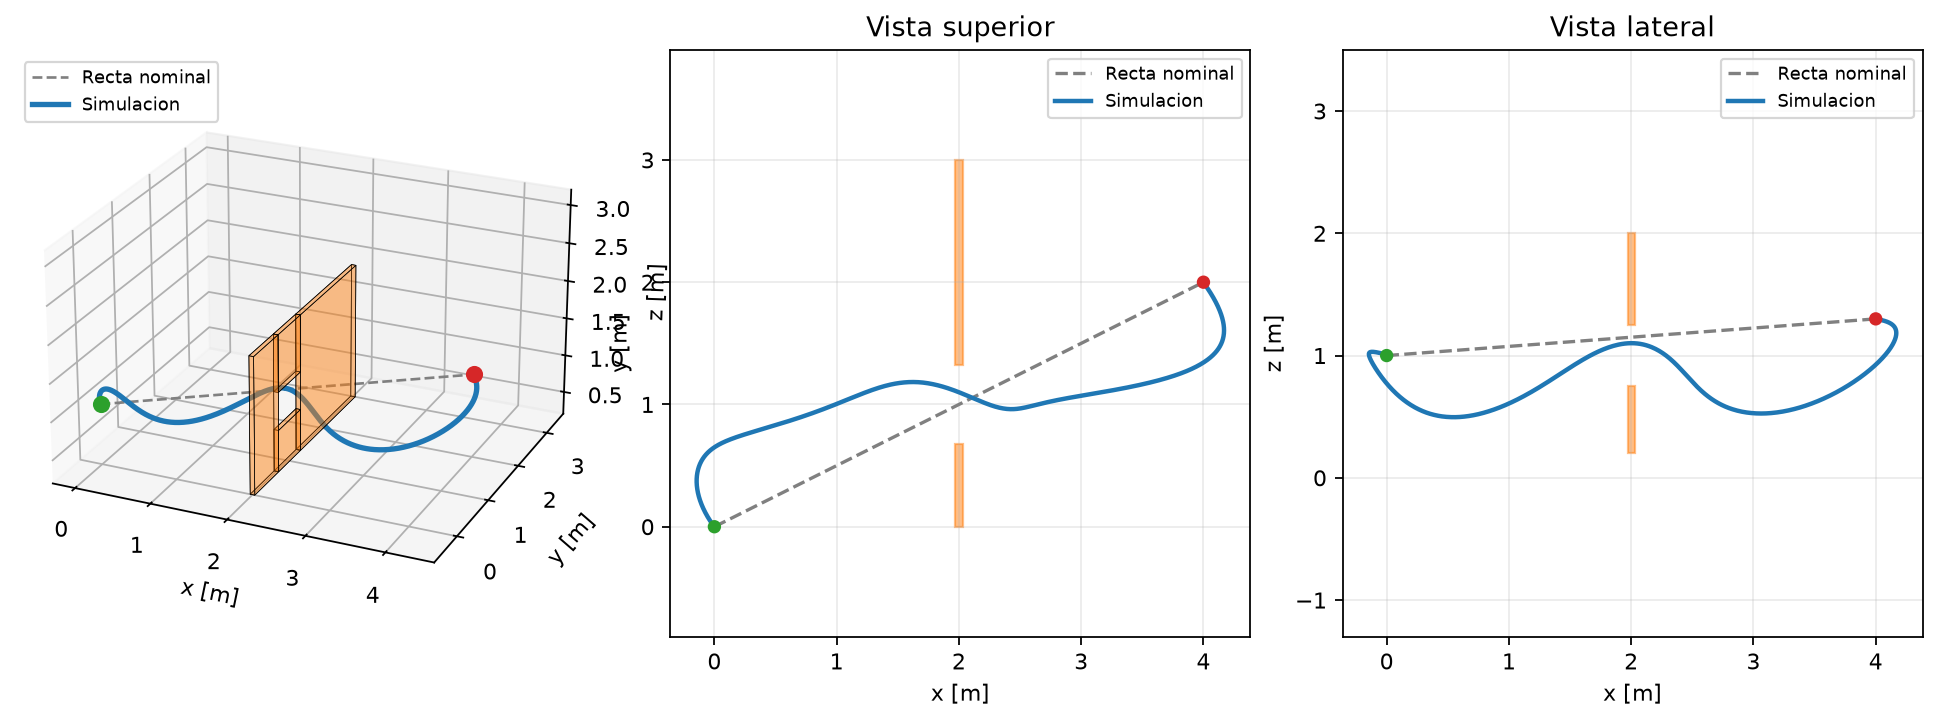
\includegraphics[width=\linewidth]{p2_trayectoria.png}
\end{column}
\begin{column}{0.44\textwidth}
\begin{tbox}{Comportamiento Cinemático}
\scriptsize
\begin{itemize}
\item El dron se desvía de la linea recta nominal: desciende inicialmente para ganar velocidad y luego se nivela a la altura del orificio ($z \approx 1.1$\,m).
\item Tras cruzar el orificio invertido, recupera la posicion horizontal y gira en yaw hacia los $90^\circ$ solicitados.
\item Llegada en reposo suave a $\bp_f = (4, 2, 1.3)$\,m.
\end{itemize}
\end{tbox}
\end{column}
\end{columns}
\src{Animacion: \href{https://github.com/LEKamt/rav_ec3/blob/7780e7d0c8741acd9c4335f4ed9dffac1bd24fd3/report/figures/p2_snap_roll.gif}{p2\_snap\_roll.gif} (extremo rojo indica brazo delantero)}
\end{frame}

% ============================================================
\begin{frame}{P2: Resultados -- Holguras y Vista en el Cruce}
\begin{center}
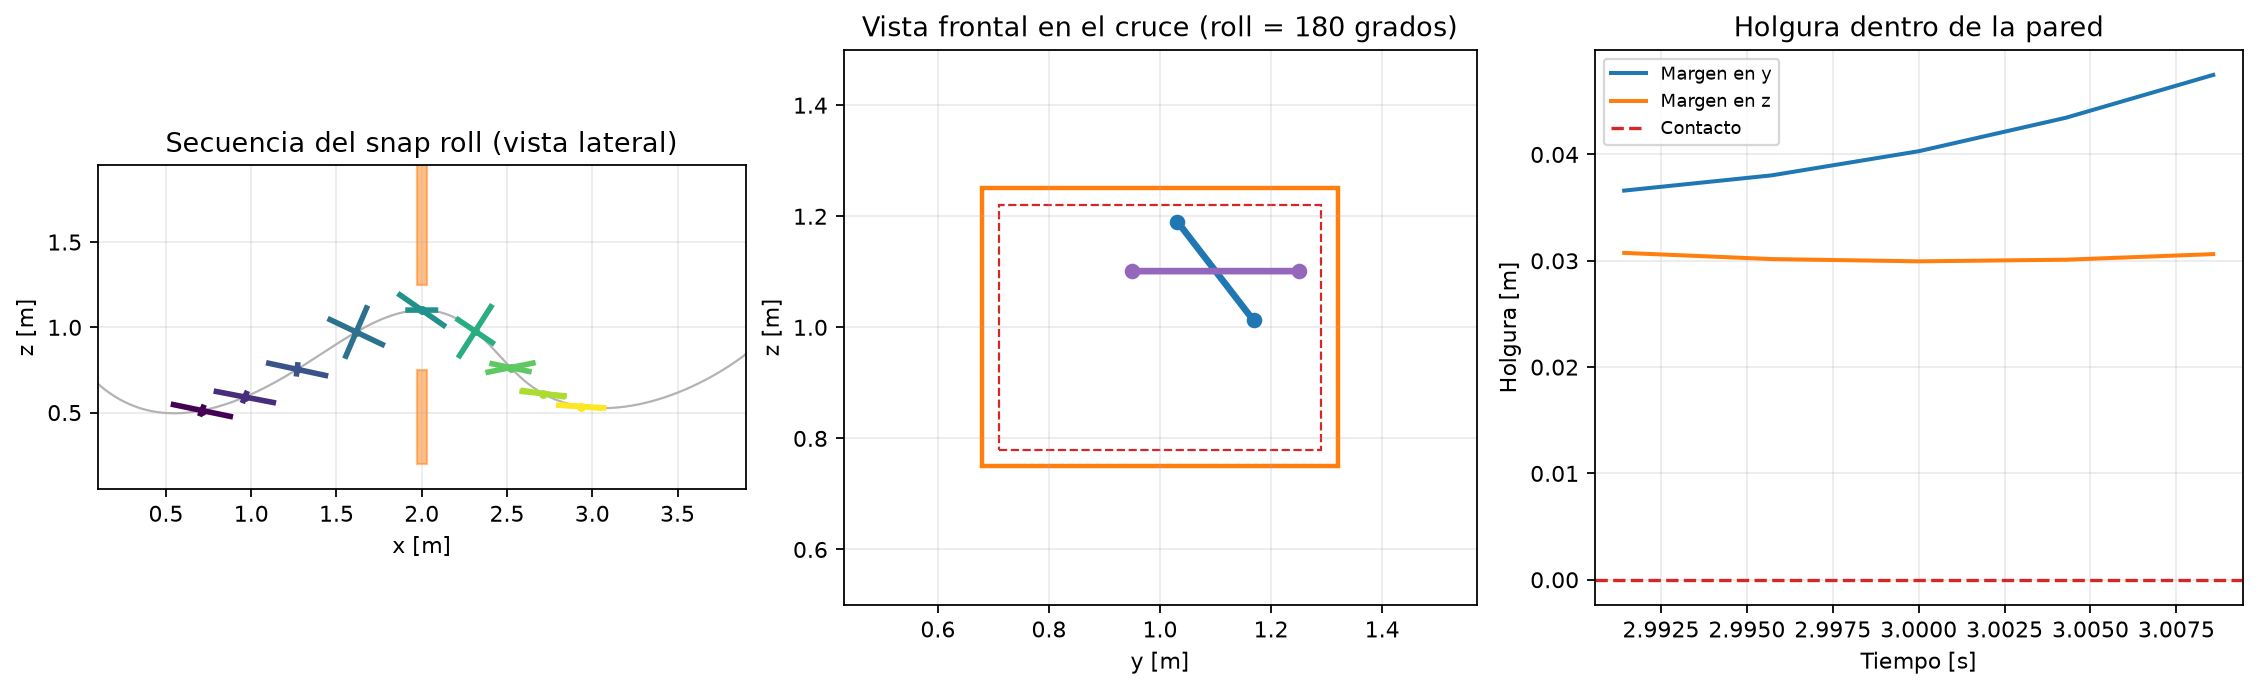
\includegraphics[width=0.88\textwidth]{p2_snap_roll_secuencia.png}
\end{center}
\begin{tbox}{Verificación de Holguras}
\scriptsize
\begin{itemize}
\item Durante el cruce de la pared, las 4 puntas de los rotores presentan márgenes de holgura positivos: $\Delta y_{\min} \approx 3.7$\,cm y $\Delta z_{\min} \approx 3.0$\,cm respecto al marco de la pared.
\item No existe colisión física durante la maniobra.
\end{itemize}
\end{tbox}
\end{frame}


% ============================================================
\begin{frame}{P2: Verificación con Integrador Continuo DOP853}
\begin{columns}[T]
\begin{column}{0.48\textwidth}
\centering
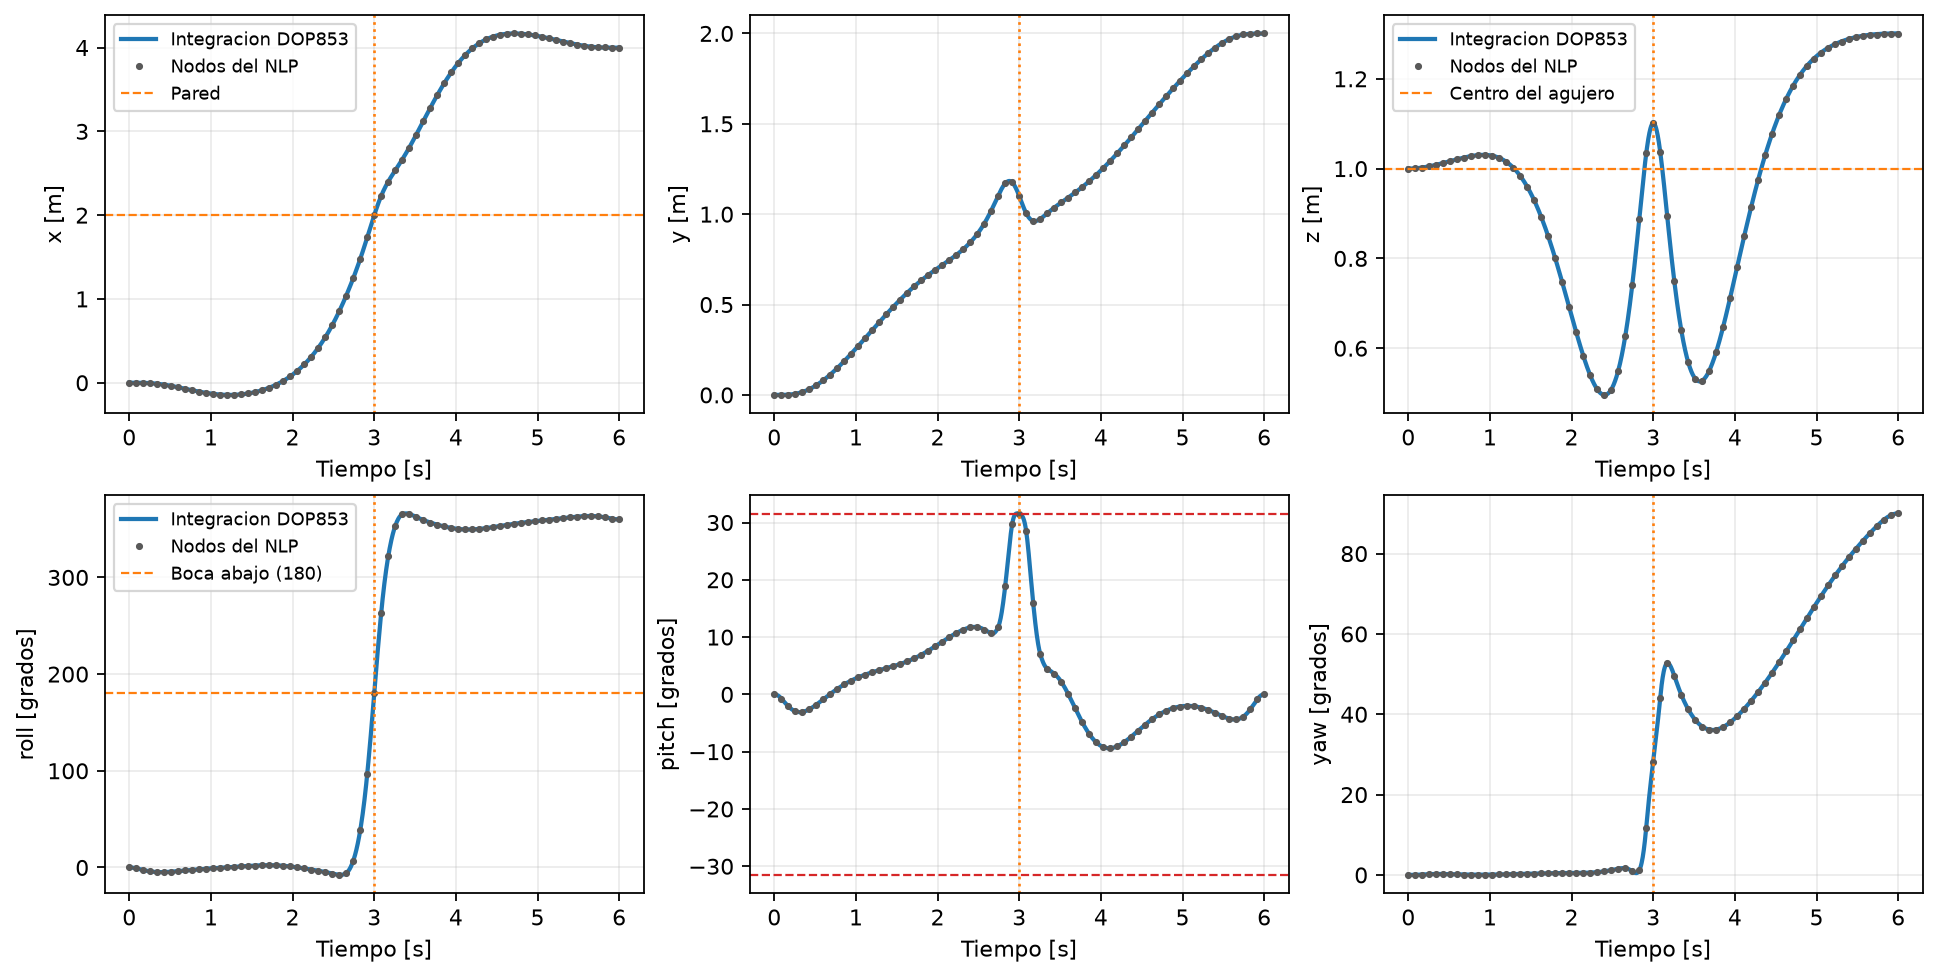
\includegraphics[width=\linewidth]{p2_estados.png}
\vskip2pt
{\tiny \textbf{Estados:} Puntos (NLP) vs Linea continua (DOP853)}
\end{column}
\begin{column}{0.48\textwidth}
\centering
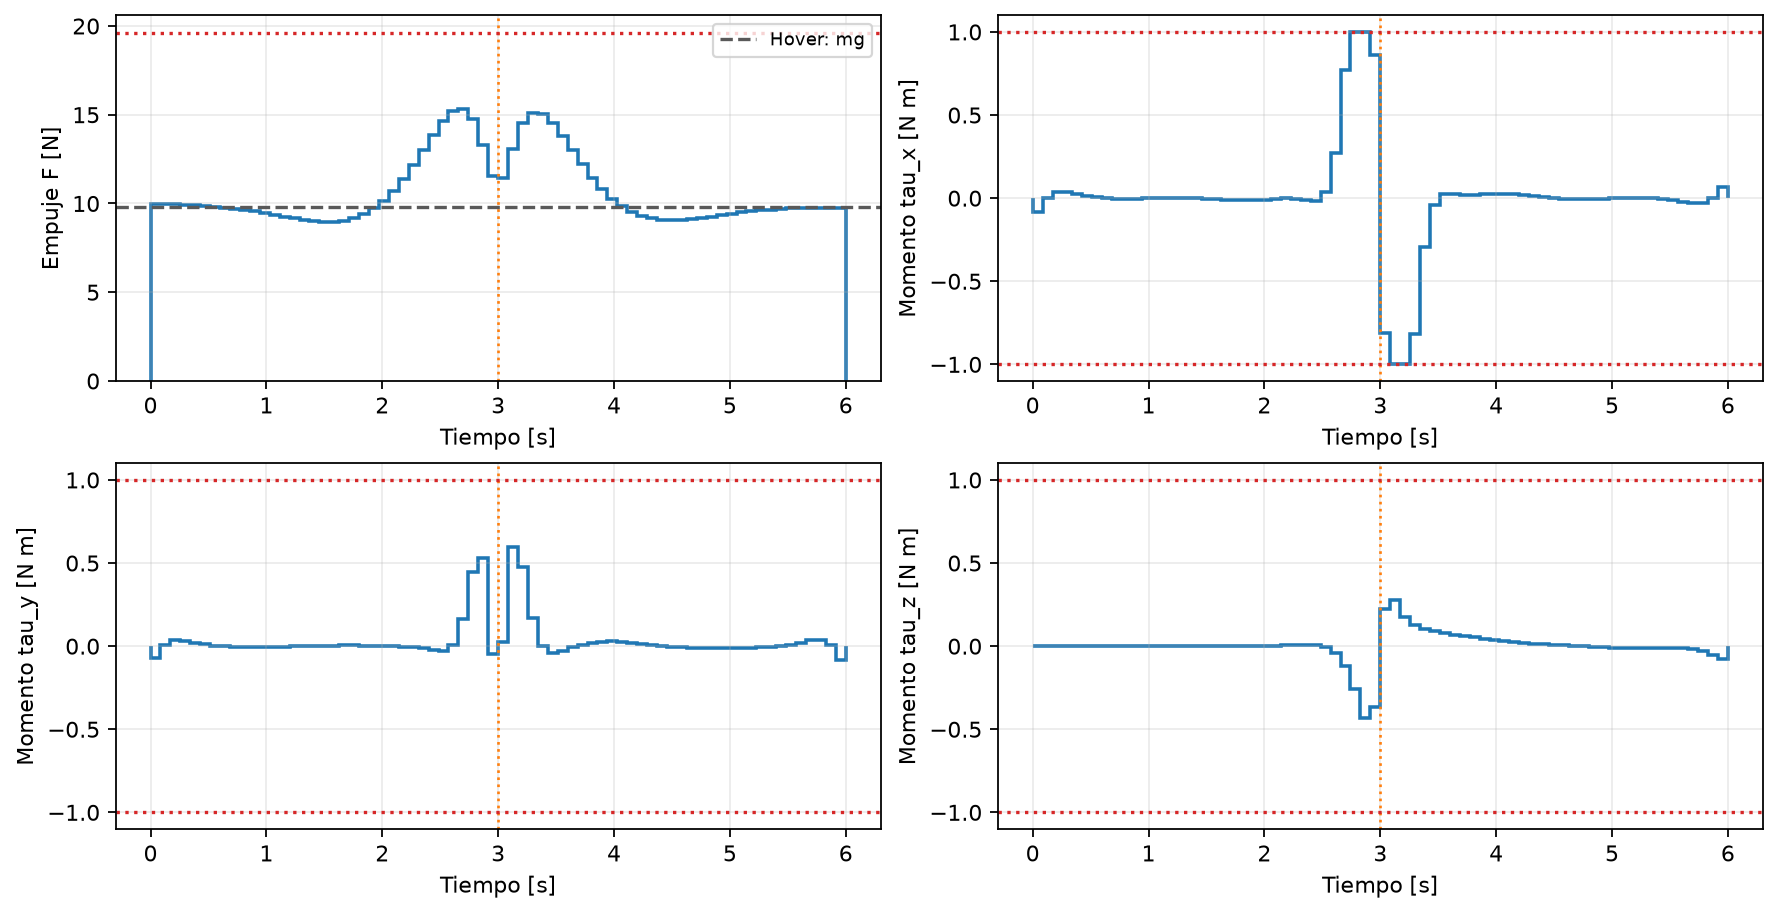
\includegraphics[width=\linewidth]{p2_controles.png}
\vskip2pt
{\tiny \textbf{Controles:} Empuje $F$ y momentos de control $\btau$}
\end{column}
\end{columns}
\vskip4pt
\begin{tbox}{Fidelidad de la Solución}
\scriptsize
\begin{itemize}
\item Coincidencia casi exacta entre la solución discreta del NLP y la integración continua con DOP853 (defectos de continuidad $< 10^{-4}$).
\item $\tau_x$ satura en $\pm 1\,\text{N}\cdot\text{m}$ (límite físico) para ejecutar el giro rápido de roll de $360^\circ$ en $1.0$\,s.
\end{itemize}
\end{tbox}
\end{frame}